\section{Drone Related Hardware}
\label{toolkitsection}
In real life, there are multiple constraints and restrictions. To successfully implement ideas, all of these limitations should be taken into consideration. Specifically, for using a deep learning-based approach on a drone, sensing systems, and communications design constraints should be investigated intensively~\cite{fraga2019review}. The hardware factors of a drone are shown in Fig~\ref{hardware}. These factors are discussed below.
\begin{figure}[h!]
\centering
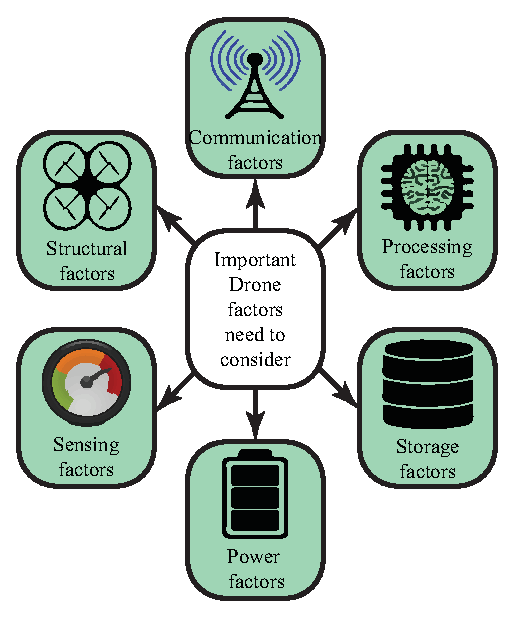
\includegraphics[width=.7\linewidth]{figure/hardware.eps}
\caption{Factors need to be considered before using drone.}
\label{hardware}
\end{figure}
\subsection{Communication Factors}
The most important part of the drone is the communication system. RFID and WIFI are the most commonly used communication protocols for drones. Another popular alternative to these protocols is Bluetooth, as Bluetooth consumes less power then WIFI. But the advantage of WIFI over Bluetooth is the high data transmission and receiving rate. But both of these protocols can not be used for long-range communication. For that purpose, cellular networks can be used. Based on the communication range, frequency bandwidth, data transmission rate, and power consumption criteria, we need to select the communication protocol. There are many communication protocols, such as Zigbee, Z-wave, NFC (narrow field communication), etc. In Table~\ref{communicationprotocol}, we have provided a few communication protocols used for drone communication.
\begin{table}[h]
\scriptsize
\centering
\caption{Wireless communication protocols for drone}
\begin{tabular}{@{}|l|l|l|l|l|@{}}
\toprule
          & Band                                                                             & Range                                                   & Data rate                                                      & \begin{tabular}[c]{@{}l@{}}Power\\ consumption\end{tabular} \\ \midrule
Wifi      & \begin{tabular}[c]{@{}l@{}}900MHz, 2.4GHz, 3.65\\ GHz, 5GHz, 5.9GHz\end{tabular} & 100m                                                    & \begin{tabular}[c]{@{}l@{}}2Mbps to\\ 54Mbps\end{tabular}      & high                                                        \\ \midrule
Bluetooth & 2.4GHz                                                                           & 250m                                                    & upto 2Mbps                                                     & low                                                         \\ \midrule
Zigbee    & 2.4GHz                                                                           & \begin{tabular}[c]{@{}l@{}}10m to\\ 100m\end{tabular}   & 100kbps                                                        & very low                                                    \\ \midrule
Z-wave    & 900MHz                                                                           & 30m                                                     & 100kbps                                                        &                                                             \\ \midrule
6LoWPAN   & \begin{tabular}[c]{@{}l@{}}2.4GHz or\\ 900MHz\end{tabular}                       & \begin{tabular}[c]{@{}l@{}}10m to\\ 100m\end{tabular}   & 250kbps                                                        & low                                                         \\ \midrule
RF        & \begin{tabular}[c]{@{}l@{}}starts from KHz and\\ ranges till GHz\end{tabular}    & \begin{tabular}[c]{@{}l@{}}10cm to\\ 200m\end{tabular}  & \begin{tabular}[c]{@{}l@{}}depends on\\ frequency\end{tabular} &                                                             \\ \midrule
Cellular  & 900MHz to 2100MHz                                                                & \begin{tabular}[c]{@{}l@{}}35km to\\ 200km\end{tabular} & \begin{tabular}[c]{@{}l@{}}35Kbps to\\ 10Mbps\end{tabular}     & Very high                                                   \\ \midrule
NB-IOT    & 200KHz                                                                           & 10Km                                                    & 250kbps                                                        & low                                                         \\ \midrule
5G        & 6GHz                                                                             & 500m                                                    & 1Gbps                                                          & Very high                                                   \\ \midrule
NFC       & 13.56MHz                                                                         & 10cm                                                    & \begin{tabular}[c]{@{}l@{}}100kbps to\\ 420kbps\end{tabular}   & low                                                         \\ \midrule
LoRaWAN   & 2.4GHz                                                                           & \begin{tabular}[c]{@{}l@{}}2km to\\ 5km\end{tabular}    & \begin{tabular}[c]{@{}l@{}}0.3kbps to\\ 50kbps\end{tabular}    & Very low                                                    \\ \bottomrule
\end{tabular}
\label{communicationprotocol}
\end{table}




% \begin{table}[h]
% \centering
% \caption{Wireless communication protocols for drone}
% \begin{tabular}{|l|l|l|l|l|}
% \hline
%             & Band                                                                                  & Range                                                           & Data rate                                                      & \begin{tabular}[c]{@{}l@{}}Power\\ consu-\\ mption\end{tabular} \\ \hline
% WIFI        & \begin{tabular}[c]{@{}l@{}}900MHz, 2.4GHz,\\3.65GHz, 5GHz,\\ 5.9GHz\end{tabular}                            & 100m                                                        & \begin{tabular}[c]{@{}l@{}}2Mbps\\ to\\ 54Mbps\end{tabular}    & high                                                            \\ \hline
% Bluetooth   & 2.4GHz                                                                                & 250m                                                       & \begin{tabular}[c]{@{}l@{}}upto\\ 2Mbps\end{tabular}           & low                                                             \\ \hline
% Zigbee      & 2.4GHz                                                                                & \begin{tabular}[c]{@{}l@{}}10m\\ to\\ 100m\end{tabular}   & 100kbps                                                        & \begin{tabular}[c]{@{}l@{}}very\\ low\end{tabular}              \\ \hline
% Z-wave      & 900MHz                                                                                & 30m                                                                                                          & 100kbps                                                        &                                                                 \\ \hline
% 6LoWPAN     & \begin{tabular}[c]{@{}l@{}}2.4GHz\\ or\\ 900MHz\end{tabular}                          &        \begin{tabular}[c]{@{}l@{}}10m\\ to\\ 100m\end{tabular}                                                   &     250kbps                                                           & low                                                             \\ \hline
% RF          & \begin{tabular}[c]{@{}l@{}}starts\\ from\\ KHz\\ and\\ ranges\\ till GHz\end{tabular} & \begin{tabular}[c]{@{}l@{}}10cm\\ to\\ 200m\end{tabular}                                                         & \begin{tabular}[c]{@{}l@{}}depends\\ on\\ frequency\end{tabular}       &                                                                 \\ \hline
% Cellular    & \begin{tabular}[c]{@{}l@{}}900MHz\\ to\\ 2100MHz\end{tabular}                         & \begin{tabular}[c]{@{}l@{}}35km\\ to\\ 200km\end{tabular} &                                                          \begin{tabular}[c]{@{}l@{}}35Kbps\\ to\\ 10Mbps\end{tabular}   &       \begin{tabular}[c]{@{}l@{}}Very\\ high\\\end{tabular}        \\ \hline
% NB-IOT      &         200KHz                                                                              & 10Km                                                                                                               & 250kbps                                                        & low                                                             \\ \hline
% 5G          & 6GHz                                                                                  &        500m                                                                                                            & 1Gbps                                                          &    \begin{tabular}[c]{@{}l@{}}Very\\ high\\\end{tabular}                                                              \\ \hline
% NFC         & 13.56MHz                                                                              & 10cm                                                                                                              & \begin{tabular}[c]{@{}l@{}}100kbps\\ to\\ 420kbps\end{tabular} &                     low                                            \\ \hline
% LoRaWAN     & 2.4GHz                                                                                & \begin{tabular}[c]{@{}l@{}}2km\\ to\\ 5km\end{tabular}                                                           & \begin{tabular}[c]{@{}l@{}}0.3kbps\\ to\\ 50kbps\end{tabular}  &   \begin{tabular}[c]{@{}l@{}}Very\\ low\\\end{tabular}                                                              \\ \hline
% %LTE-M       &                                                                                       &                                                           &                                                         & \begin{tabular}[c]{@{}l@{}}100kbps\\ to\\ 375kbps\end{tabular} &                                                                 \\ \hline
% \end{tabular}
% \label{communicationprotocol}
% \end{table}

\subsection{Sensor Factors}
Sensors play a crucial role in drone navigation and data capture. Those sensors help the drone to collect data from the surroundings. Using this knowledge, a drone can maintain its positions, decide how fast it is moving, and avoid barriers. Commonly used drone sensors are mentioned below.

\textbf{RGB camera:} 
The most commonly attached sensor in a drone is an RGB camera. An RGB camera is required to provide drone pilots with feedback. Besides, a range of creative and realistic applications are found with drone cameras these days. Among them, autonomous navigation, wildlife surveillance, weather forecasting, archaeological surveys, aerial photography are notable. Depending on the price, drone cameras can vary in quality and size.

\textbf{Thermal camera:}
A thermal camera can transform the drone into a versatile device that can be used in many sectors, such as quarrying, energy monitoring, health inspection, firefighting, etc. The thermal camera uses vision imaging technique that can sense and transform heat coming from virtually all objects and materials into photographs. 

\textbf{Gyroscope:}
Gyroscope is inexpensive and easy enough to fit into even inexpensive mini-drones. The gyroscopes work on the principle of angular momentum conservation. This device is used to measure or maintain orientation.

\textbf{Accelerometers:}
A drone's accelerometer operates in tandem with its gyroscope to determine changes in the drone's position and motion. The working principle of an accelerometer is based on the piezoelectric effect. A gyroscope can read rotational movements, whereas an accelerometer is better able to read linear motions along any axis. 

\textbf{Tilt Sensor:}
The tilt sensor is a hybrid sensor that consists of a gyroscope and an accelerometer. The tilt sensor can provide feedback into the flight-control device to maintain level flight.

\textbf{Barometer:}
Barometers are atmospheric pressure measuring instruments. By using the atmospheric pressure, a drone can determine it's altitude from the ground. 

\textbf{GPS:}
Global Positioning System is an essential part of commercial drones. It plays an important role in the field of autonomous navigation. The GPS sensor communicates with the GPS satellite and detects the position based on the satellite. Then the 3D position of the drone within a given geospatial reference network is calculated by triangulating the position of the drone with respect to the various GPS satellites.

\textbf{Magnetometer:}
A magnetometer, as its name suggests, measures the direction and force of a magnetic field. Using a magnetometer, a drone can determine the strength of the magnetic and electric field and change its route consequently.

\textbf{IMU:}
Inertial Measurement Units or also known as IMU is a combined package, that consists of accelerometers, magnetometers, and gyroscopes.

\textbf{Sonar Sensor:}
The Sonar sensor uses sound waves to detect the distance between an object and the drone. By using multiple sonar sensors, the drone can avoid obstacles towards its path.

\subsection{Other Factors}
Beside embedded sensors and communication systems, we need to consider a few other factors before buying a drone. Weight, size, and maximum payload of a drone is the most important parameters because flight time mostly depends on these specifications. A professional parcel delivering drone on average can lift weighing around 40 lbs. On the other hand, the average flight time of the majority of commercial drones is 20-30 minutes. Though flight time can be increased by using a powerful battery, it must be noted that the higher the battery strength, the heavier it becomes. The bottlenecks of battery technology are Li-ion, LiPolymer, etc. However, research is still going on for a long-life battery with reduced weight. The other two important specifications are the controlling system and the storage system. Commonly used microprocessors are based on ARM architecture. Considering all the criteria mentioned above, a list of drones used for the educational research purpose is provided in Table~\ref{dronetable}.
\begin{table}[h]
\scriptsize
\centering
\caption{List of common drones used for research}
\begin{tabular}{@{}|l|l|l|l|l|l|@{}}
\toprule
Drone Name                                                           & \begin{tabular}[c]{@{}l@{}}Flight\\ Time\end{tabular} & Range & Camera                                                     & Other sensors                                                                        & Price (\$) \\ \midrule
DJI Mavic Pro                                                        & 27 min                                                & 7 km  & 12 MP                                                      &                                                                                      & 899        \\ \midrule
DJI Spark                                                            & 16 min                                                & 2 km  & 12 MP                                                      &                                                                                      & 455        \\ \midrule
\begin{tabular}[c]{@{}l@{}}DJI Phantom 4\\ Pro\end{tabular}          & 30 min                                                & 7 km  & 20 MP                                                      & IR sensor                                                                            & 1729       \\ \midrule
\begin{tabular}[c]{@{}l@{}}DJI Phantom 4\\ Advanced\end{tabular}     & 30 min                                                & 7 km  & 20 MP                                                      &                                                                                      & 900        \\ \midrule
DJI Inspire 2                                                        & 27 min                                                & 7 km  & \begin{tabular}[c]{@{}l@{}}No built-\\ in cam\end{tabular} & IR sensor                                                                            & 3499       \\ \midrule
\begin{tabular}[c]{@{}l@{}}DJI Matric\\ 100\end{tabular}             & 40 min                                                & 5 km  & \begin{tabular}[c]{@{}l@{}}No built-\\ in cam\end{tabular} & \begin{tabular}[c]{@{}l@{}}Pressure, GPS,\\ Magnetometer,\\ Ultra sonic\end{tabular} & 3299       \\ \midrule
\begin{tabular}[c]{@{}l@{}}YUNEEC\\ TYPHOON\end{tabular}             & 22 min                                                & 1 km  & 12 MP                                                      & Sonar sensor                                                                         & 1199       \\ \midrule
\begin{tabular}[c]{@{}l@{}}Parrot ANAFI\\ Thermal Drone\end{tabular} & 26 min                                                & 4 km  & 21 MP                                                      & \begin{tabular}[c]{@{}l@{}}GPS, Barometer,\\ Magnetometer,\\IMU\end{tabular}          & 1900       \\ \midrule
\begin{tabular}[c]{@{}l@{}}Parrot AR\\ Drone 2.0\end{tabular}        & 12 min                                                & 50 m  & HD                                                         &                                                                                      & 299        \\ \midrule
\begin{tabular}[c]{@{}l@{}}Parrot Bebop\\ 2.0\end{tabular}           & 25 min                                                & 2 km  & 14 MP                                                      & \begin{tabular}[c]{@{}l@{}}Pressure, GPS,\\ Magnetometer,\\ Ultra sonic\end{tabular} & 499        \\ \bottomrule
\end{tabular}
\label{dronetable}
\end{table}

% \begin{table*}[h]
% \scriptsize
% \centering
% \caption{List of common drones used for research}
% \begin{tabular}{|l|l|l|l|l|l|}
% \hline
% Drone Name                 & Flight Time & Range & Camera                                                    & Other sensors                                                                       & Price (\$) \\ \hline
% DJI Mavic Pro              & 27 min      & 7 km  & 12 MP                                                     &                                                                                     & 899        \\ \hline
% DJI Spark                  & 16 min      & 2 km  & 12 MP                                                     &                                                                                     & 455        \\ \hline
% DJI Phantom 4 Pro          & 30 min      & 7 km  & 20 MP                                                     & IR sensor                                                                           & 1729       \\ \hline
% DJI Phantom 4 Advanced     & 30 min      & 7 km  & 20 MP                                                     &                                                                                     & 900        \\ \hline
% DJI Inspire 2              & 27 min      & 7 km  & \begin{tabular}[c]{@{}l@{}}No built-in  cam\end{tabular} & IR sensor                                                                           & 3499       \\ \hline
% DJI Matric 100             & 40 min      & 5 km  & \begin{tabular}[c]{@{}l@{}}No built-in  cam\end{tabular} & \begin{tabular}[c]{@{}l@{}}Pressure, GPS, Magnetometer, Ultra sonic\end{tabular} & 3299       \\ \hline
% YUNEEC TYPHOON H           & 22 min      & 1 km  & 12 MP                                                     & Sonar sensor                                                                        & 1199       \\ \hline
% Parrot ANAFI Thermal Drone & 26 min      & 4 km  & 21 MP                                                     & \begin{tabular}[c]{@{}l@{}}GPS, Barometer, Magnetometer, IMU\end{tabular}         & 1900       \\ \hline
% Parrot AR Drone 2.0        & 12 min      & 50 m  & HD                                                        &                                                                                     & 299        \\ \hline
% Parrot Bebop 2.0           & 25 min      & 2 km  & 14 MP                                                     & \begin{tabular}[c]{@{}l@{}}Pressure, GPS, Magnetometer, Ultra sonic\end{tabular} & 499        \\ \hline
% \end{tabular}
% \label{dronetable}
% \end{table*}

%maybe table na top producing company https://www.businessinsider.com/drone-manufacturers-companies-invest-stocks